\chapter{Implementación}
En este capítulo se va a abordar la implementación del sistema. Para ello, en
primer lugar, se van a explicar las herramientas y tecnologías que se han utilizado
y el porqué de su elección. En segundo lugar, se explicará la implementación de la
base de datos, se mostrará el diagrama de clases y, por último, se explicará la
implementación de la aplicación, tanto del backend como del frontend.

\section{Herramientas y tecnologías}
En este apartado se van a explicar las herramientas y tecnologías utilizadas
para el desarrollo de la aplicación.

\subsection{Control de versiones}
Para realizar un seguimiento del desarrollo de la aplicación se ha utilizado la
herramienta de control de versiones \textit{Git} \cite{git}, que permite llevar un
control de los cambios realizados en el código fuente de la aplicación. Además, estos
cambios se han ido subiendo a la plataforma \textit{GitHub} \cite{github}.

Para seguir una estructura de los commits que se van realizando, se han ido escribiendo
los mensajes de commit con el formato "\texttt{<stack>} - \texttt{<mensaje>}", donde
\texttt{<stack>} es \textit{SERVER} o \textit{CLIENT} dependiendo de si el commit afecta
al backend o al frontend de la aplicación, y \texttt{<mensaje>} es la descripción de los
cambios que se han realizado.

En la figura \ref{fig:commits} se puede ver un ejemplo de una captura sacada
del listado de commits realizados en el repositorio de \textit{GitHub} \cite{github}.

\begin{figure}[H]
  \centering
  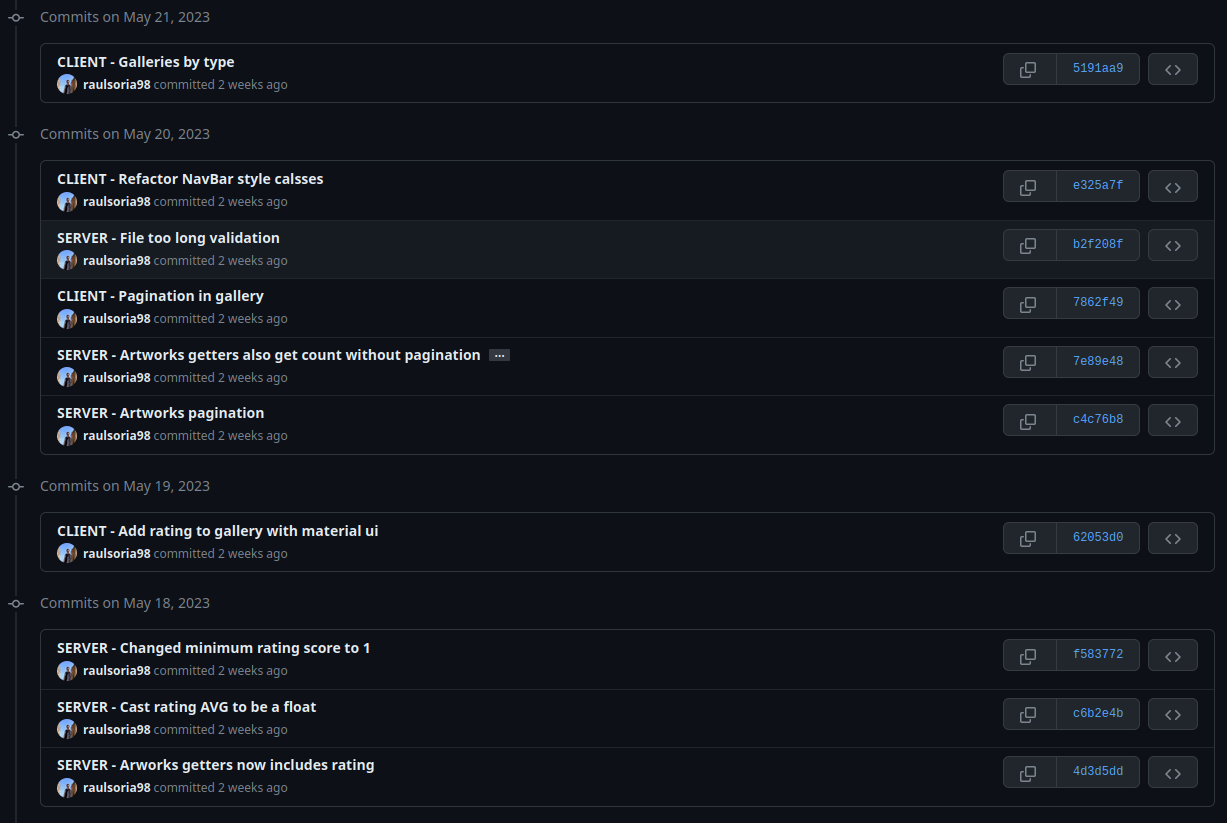
\includegraphics[width=1\textwidth]{commits}
  \caption{Ejemplo de mensajes de commit}
  \label{fig:commits}
\end{figure}

\subsection{Base de datos}
Para la base de datos había que elegir en primer lugar entre una base de datos
relacional o una base de datos no relacional.

En este artículo \cite{relational-vs-non-relational} se explica la diferencia entre
un tipo de base de datos y otro, las ventajas que tiene cada una y en qué casos es
más recomendable utilizar una u otra.

En el caso de nuestra aplicación, se ha optado por utilizar una base de datos relacional
ya que, aunque la base de datos no va a ser muy grande, sí que va a tener una estructura
bien definida con relaciones fuertes entre las tablas.

También es necesario elegir el gestor de base de datos que se va a utilizar, ya que
existen varios gestores de bases de datos relacionales. En nuestro caso se ha optado
por utilizar \textit{MySQL} \cite{mysql} ya que es el gestor de bases de datos
relacionales más utilizado y es el que más conozco personalmente.

\subsection{Backend}
Para el desarrollo del backend de la aplicación se ha utilizado \textit{Node.js}
\cite{nodejs} que es un entorno de ejecución de JavaScript. Se ha elegido este
entorno porque quería aprender a utilizarlo dada su popularidad y porque así podría
utilizar JavaScript tanto en el backend como en el frontend. Este último punto
hizo que descartara utilizar otros frameworks como \textit{Django} \cite{django}
o \textit{Ruby on Rails} \cite{ruby-on-rails}.

Como framework complementario a \textit{Node.js} se ha utilizado \textit{Express}
\cite{express} que facilita la creación de aplicaciones web y de APIs en \textit{Node.js}.

\subsection{Frontend}
Para el desarrollo del frontend de la aplicación se barajaron varias opciones.
En primer lugar, se pensó en utilizar \textit{Angular} \cite{angular} ya que es un
framework bastante popular y con el que ya había trabajado anteriormente. Sin embargo,
se descartó esta opción porque, como explican en este artículo \cite{angular-vs-react},
este es un framework muy completo y pensado para aplicaciones grandes donde prima el
trabajo en equipo ya que su estructura es fija y esto la hace más compleja. Mientras
que \textit{React} \cite{react} es una biblioteca más sencilla y flexible que permite
crear aplicaciones pequeñas como la nuestra de manera sencilla y sin una gran curva de
aprendizaje.

También se barajó la opción de utilizar \textit{Vue.js} \cite{vuejs} ya que es una
librería de la que también había oído hablar y que también usa JavaScript.
Como comentan en este otro artículo \cite{vuejs-vs-react}, \textit{Vue.js} \cite{vuejs}
también es una librería bastante sencilla y ligera, cuyos módulos se pueden ir añadiendo
según se vayan necesitando. Sin embargo, se descartó esta opción porque, aunque
\textit{Vue.js} \cite{vuejs} es más sencillo que \textit{React} \cite{react}, este
último tiene mayor rendimiento, además, me llamaba más la atención y quería aprender a
utilizarlo.


\section{Implementación de la base de datos}
Para la implementación de la base de datos \textit{MySQL} \cite{mysql} se ha utilizado
\textit{Sequelize} \cite{sequelize} que es un ORM (Object-Relational Mapping) para
\textit{Node.js} \cite{nodejs} que permite trabajar con bases de datos relacionales
como la que se ha utilizado en este proyecto.

Tal y como se explica en este artículo \cite{orm}, \textit{'Un ORM (Object Relational
Mapping o Mapeo Objeto-Relacional en castellano) es una herramienta que nos permite mapear, o lo
que es lo mismo, convertir los objetos de tu aplicación a un formato adecuado para ser
almacenados en cualquier base de datos, creándo para ello una base de datos virtual
donde los datos disponibles en nuestra aplicación quedan vinculados con la base de datos
final.'}

Con \textit{Sequelize} \cite{sequelize} se define la conexión a la base de datos como se
puede ver en el código de la imágen \ref{fig:sequelize-db} correspondiente al archivo
\texttt{config/db.js}. Creando un objeto \texttt{sequelize} que servirá para,
posteriormente, realizar la conexión o definir los modelos de la base de datos. Como se
puede ver, el nombre de la base de datos, el usuario, la contraseña, el host y el puerto
se han definido en variables de entorno en un archivo \texttt{.env} para que no se vean
reflejados en el código fuente y así evitar que se suban a \textit{GitHub} \cite{github}.

\begin{figure}[H]
  \centering
  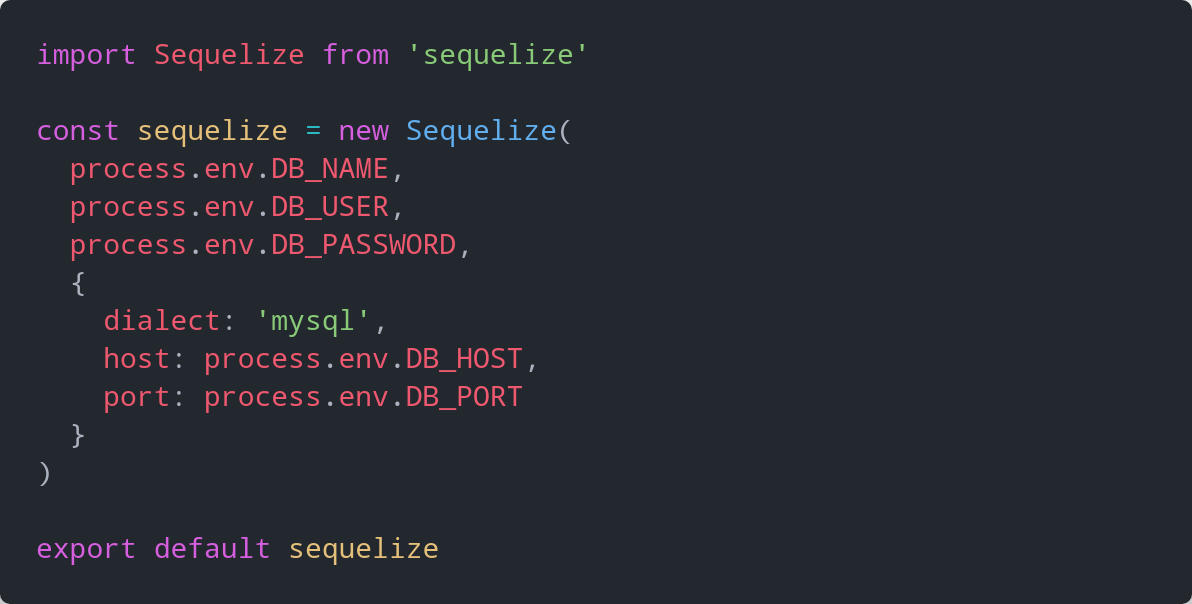
\includegraphics[width=1\textwidth]{img/sequelize-db}
  \caption{Definición de la conexión a la base de datos con \textit{Sequelize}}
  \label{fig:sequelize-db}
\end{figure}

Una vez definida la conexión a la base de datos, se realiza la conexión con la misma
mediante el método \texttt{authenticate()} como se puede ver en el código de la imágen
\ref{fig:sequelize-connect} donde se define una función de conexión que se ejecuta
cuando se inicia la aplicación.

\begin{figure}[H]
  \centering
  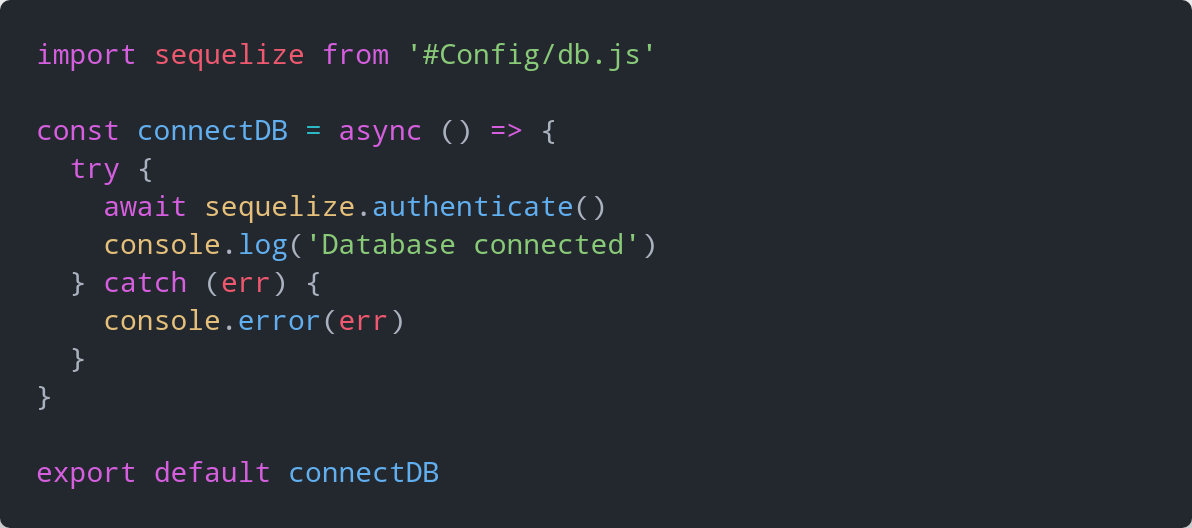
\includegraphics[width=1\textwidth]{img/sequelize-connect}
  \caption{Conexión a la base de datos con \textit{Sequelize}}
  \label{fig:sequelize-connect}
\end{figure}

Para la definición de los modelos de la base de datos se ha seguido la documentación
de \textit{Sequelize} \cite{sequelize-models} donde se explica cómo definir los modelos.
En la aplicación se han creado los archivos correspondientes
a cada modelo. Como por ejemplo el archivo \texttt{artwork.js}, cuyo código se puede ver
en la imágen \ref{fig:artwork-model}, donde se define el modelo \texttt{Artwork} con sus
atributos, validaciones y constraints.

\begin{figure}[H]
  \centering
  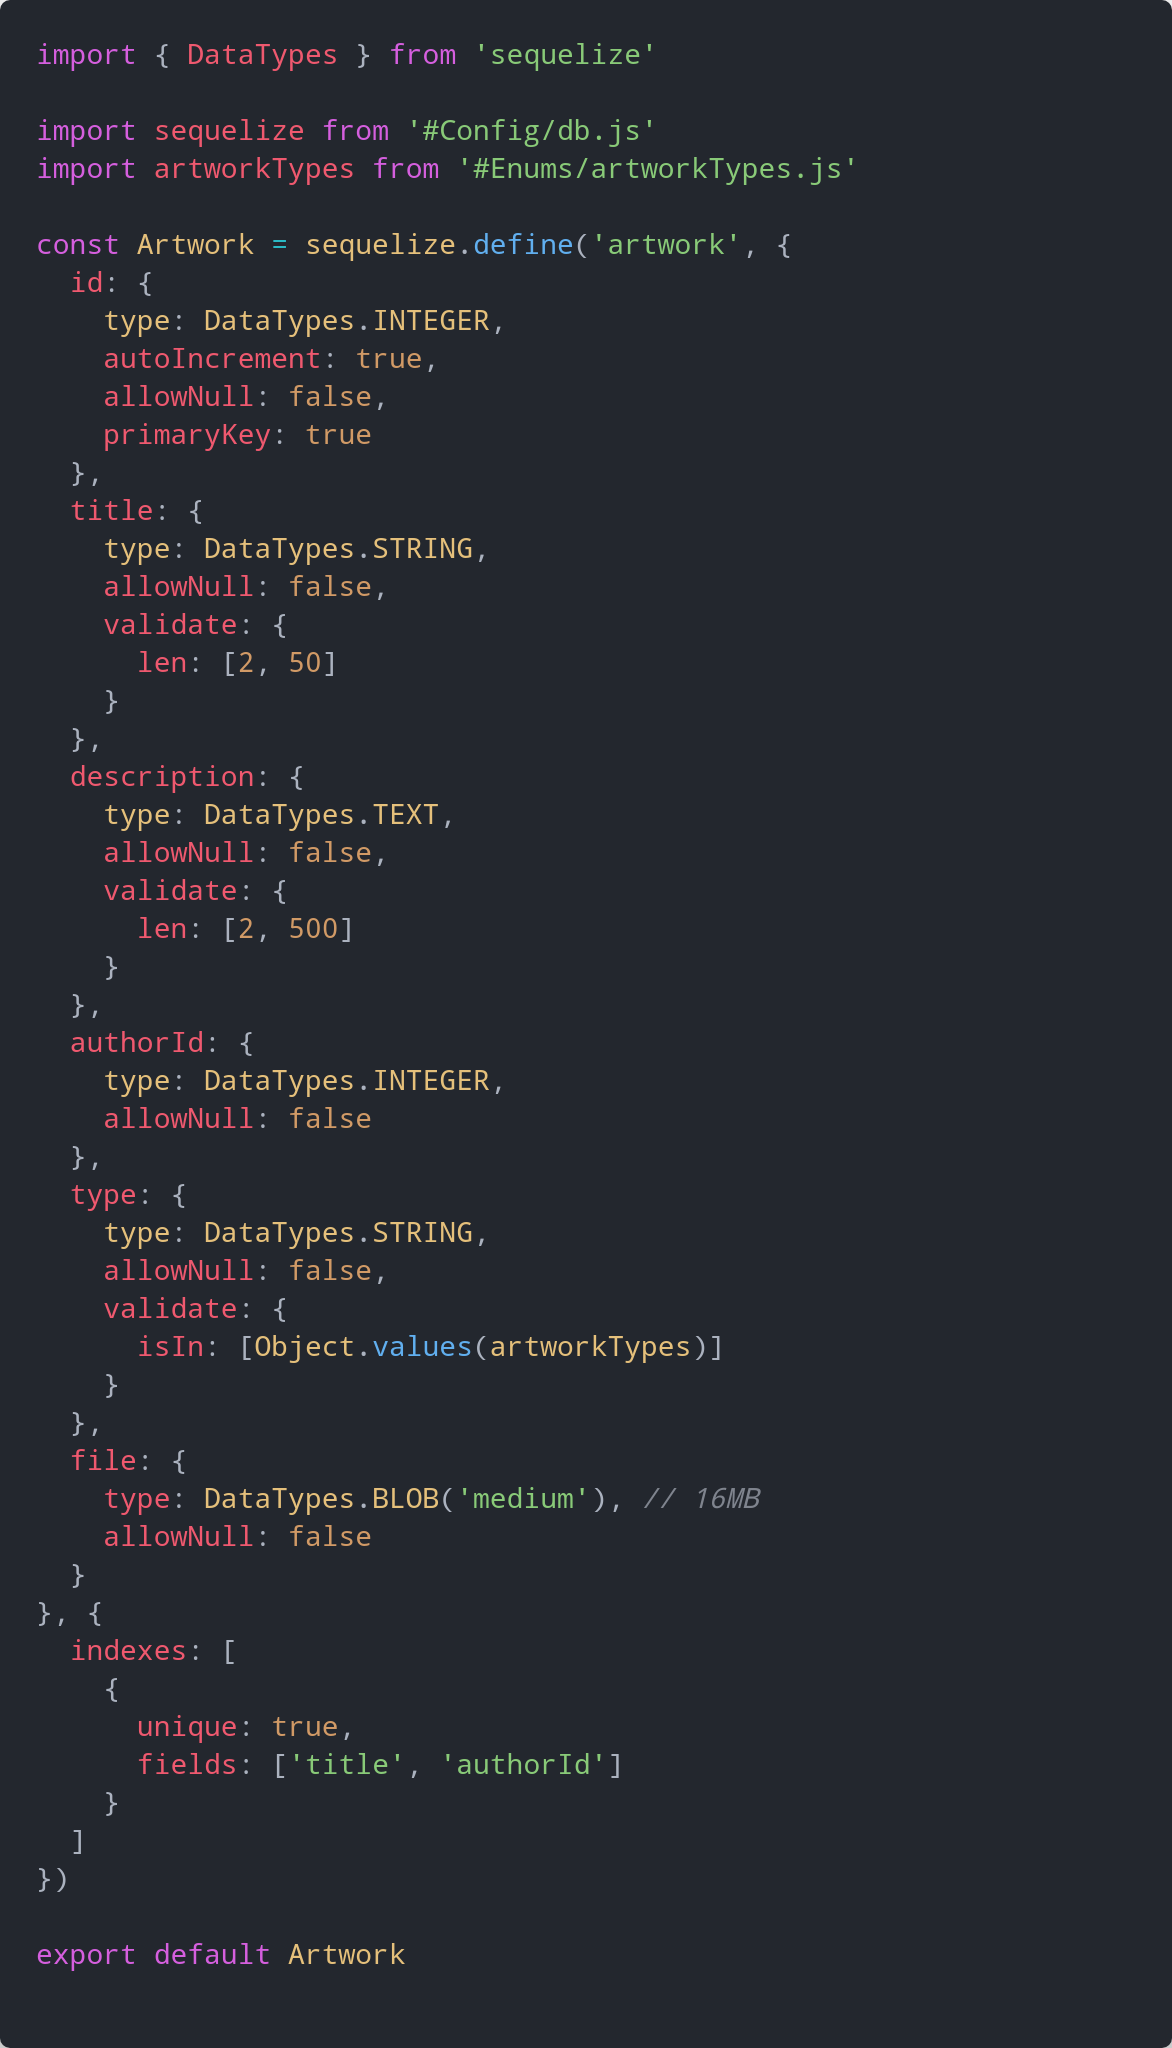
\includegraphics[width=0.8\textwidth]{img/artwork-model}
  \caption{Definición del modelo \texttt{Artwork}}
  \label{fig:artwork-model}
\end{figure}

Para las relaciones entre los distintos modelos se han seguido las instrucciones
de la documentación oficial \cite{sequelize-associations}. Se definen en una función
\texttt{associateModels} que se ejecuta justo después de realizar la conexión a la base
de datos. Como se puede ver en el código de la imágen \ref{fig:associate-models}, se
define la relación uno a muchos entre el modelo \texttt{User} y el modelo \texttt{Artwork},
la relación uno a muchos entre el modelo \texttt{User} y el modelo \texttt{Rating} y la
relación uno a muchos también, entre el modelo \texttt{Artwork} y el modelo \texttt{Rating}.

También se puede ver que se definen las claves externas de cada relación y un alias para
cada una de ellas. Esto permite realizar consultas que incluyan datos de los modelos
relacionados de manera más sencilla.

\begin{figure}[H]
  \centering
  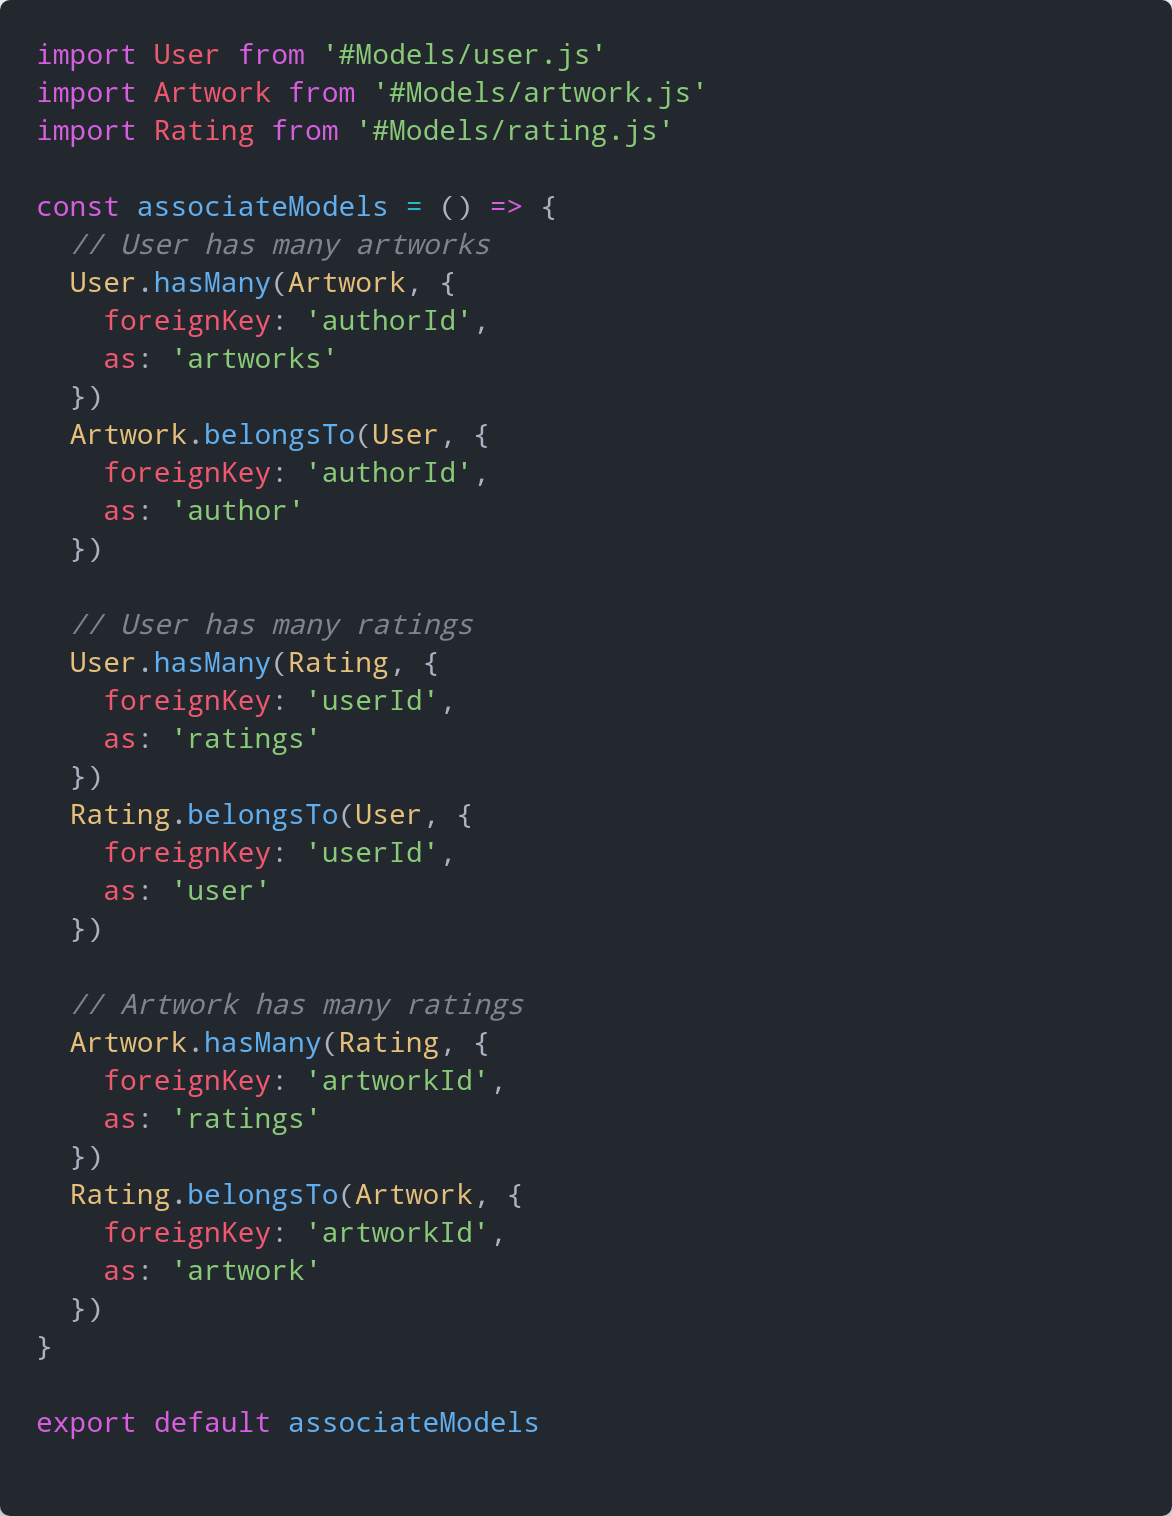
\includegraphics[width=1\textwidth]{img/associate-models}
  \caption{Definición de las relaciones entre los modelos}
  \label{fig:associate-models}
\end{figure}

Para la gestión de la base de datos se ha utilizado \textit{PhpMyAdmin} \cite{phpmyadmin}
que es una herramienta de administración de bases de datos basada en web, ofreciendo una
interfaz gráfica desde la que poder ver y gestionar los datos de la aplicación por parte
de los administradores.

Todas las contraseñas almacenadas en la base de datos se han encriptado utilizando
la librería \textit{bcrypt} \cite{bcrypt-nodejs} de \textit{Node.js} \cite{nodejs} que usa
la función de hashing \textit{bcrypt} \cite{bcrypt} basada en el cifrado Blowfish que
permite encriptar contraseñas de manera segura.

\newpage

\section{Diagrama de clases}
A continuación, en la figura \ref{fig:class-diagram}, se observa el diagrama de clases
de la aplicación. En él se pueden ver las tres clases de la aplicación: \texttt{users},
\texttt{artworks} y \texttt{ratings}. En ellas se ven sus atributos y las relaciones
entre ellas.

Como se puede ver, la clase \texttt{users} tiene una relación uno a muchos
con la clase \texttt{artworks} y la clase \texttt{ratings} tiene una relación muchos a
uno con las clases \texttt{users} y \texttt{artworks}.

\begin{figure}[H]
  \centering
  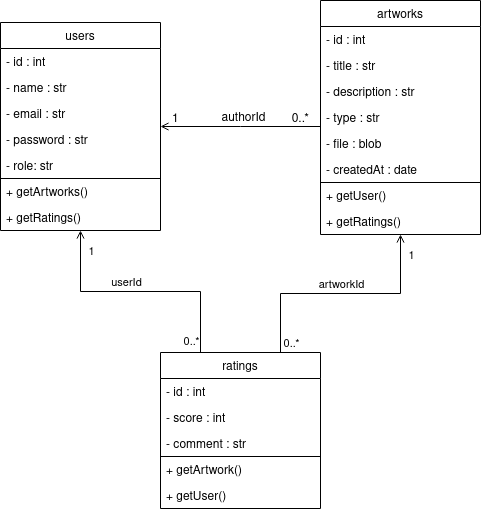
\includegraphics[width=0.9\textwidth]{diagramas/diagrama_clases}
  \caption{Diagrama de clases}
  \label{fig:class-diagram}
\end{figure}

\newpage

\section{Implementación de la aplicación}
A continuación se van a explicar los puntos más importantes de la implementación de la
aplicación, tanto en el backend como en el frontend.

\subsection{Backend}
El backend de la aplicación se ha desarrollado utilizando \textit{Node.js} \cite{nodejs}
y \textit{Express} \cite{express}. Para crear el servidor de la aplicación se ha creado
la aplicación de \textit{Express} como se muestra en el código de la imágen
\ref{fig:express-app}.

\begin{figure}[H]
  \centering
  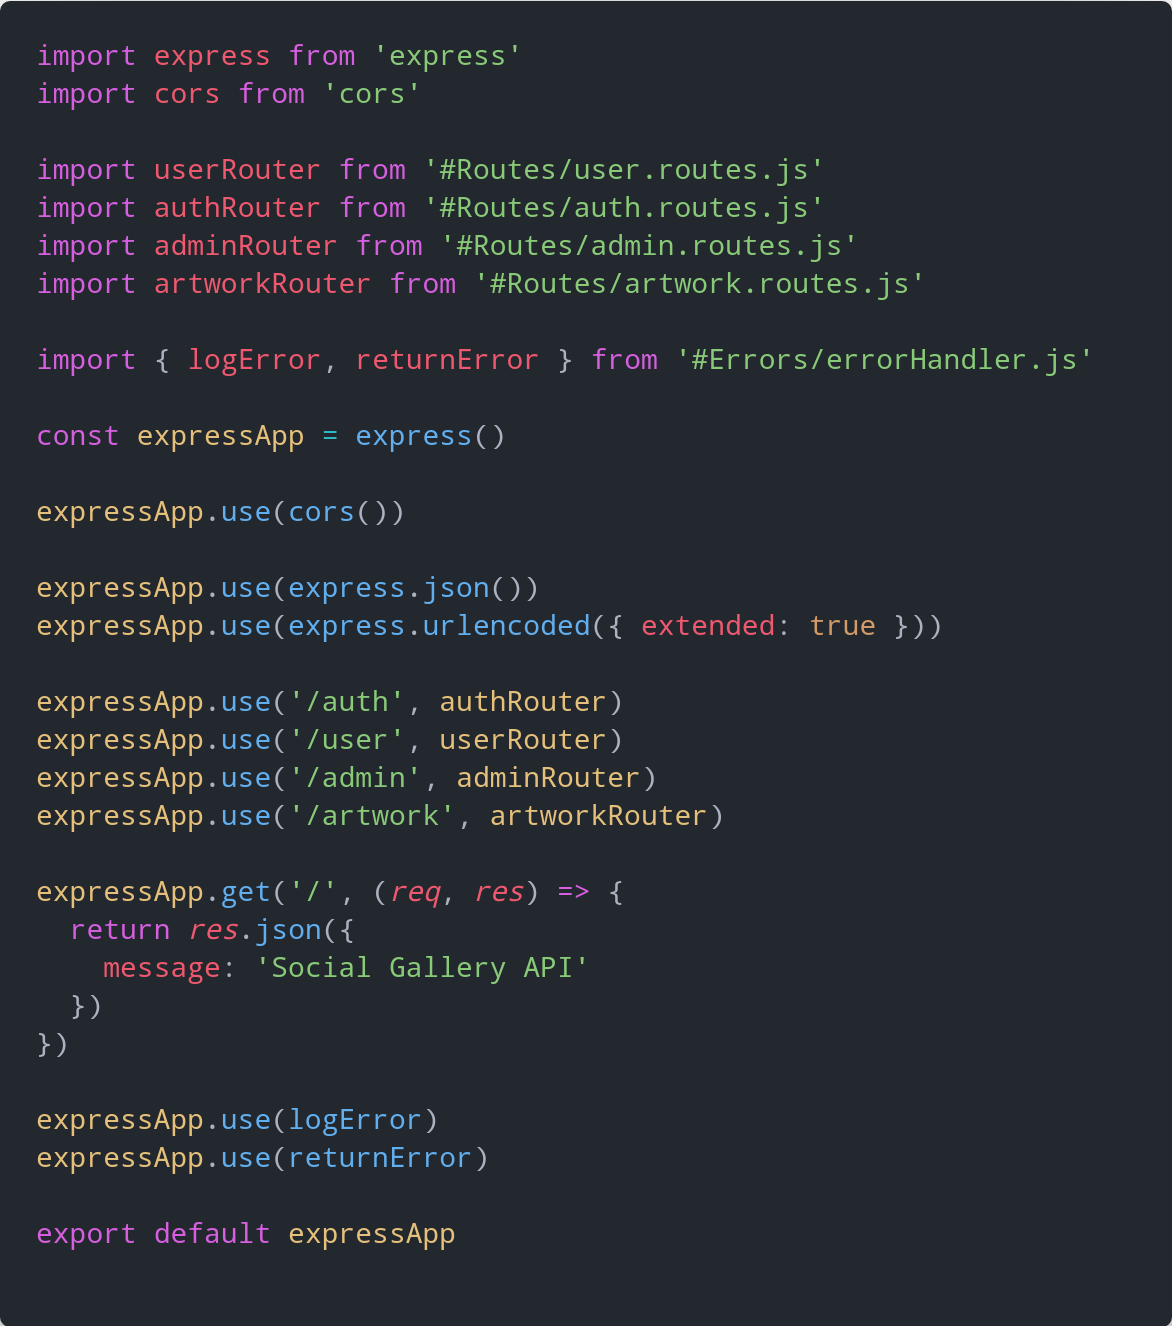
\includegraphics[width=\textwidth]{img/express-app}
  \caption{Creación de la aplicación de \textit{Express}}
  \label{fig:express-app}
\end{figure}

En él se define en primer lugar la aplicación de \textit{Express} y se le añaden los
middlewares necesarios, comenzando con el middleware \texttt{cors} \cite{express-cors}
que permite que se puedan realizar peticiones a la API desde el frontend.

A continuación se añade el middleware \texttt{express.json()} \cite{express-json}
para que la aplicación pueda recibir datos en formato \texttt{JSON}.
Después se añade el middleware de \texttt{express.urlencoded({ extended: true })}
\cite{express-urlencoded} para que la aplicación pueda recibir datos en formato
\texttt{string} o \texttt{array}.

Después se añaden los routers de la aplicación \cite{express-router} que se encargan
de gestionar las rutas de la API y llamar a las funciones correspondientes de los
controladores. También se añade la ruta por defecto que devuelve un mensaje con el
nombre de la API.

Por último, se añaden un par de middlewares más para gestionar los errores que se
puedan producir en la aplicación. Uno se encarga de mostrarlos por consola y el otro
de devolverlos en formato \texttt{JSON} y con su código de error correspondiente.

\subsubsection{Rutas}
Como se ha comentado anteriormente, los routers se encargan de gestionar las rutas
de la API y llamar a las funciones correspondientes de los controladores. Son
middlewares que agrupan rutas que tienen algo en común. En este caso, se han creado
routers para agrupar las rutas de autenticación, de los usuarios, las obras de arte
y las rutas que son para los administradores.

Como ejemplo, se puede ver el código del router de autenticación en la imágen
\ref{fig:auth-router}. En él se definen las rutas de autenticación, que son las de
inicio de sesión y registro, ambas peticiones son de tipo \texttt{POST} \cite{post-request}.
El primer parámetro que se le pasa a la función \texttt{post} de \textit{Express}
es el \texttt{path} o ruta de la petición, como se explica en la documentación
\cite{express-router}. Los siguientes parámetros son los diferentes middlewares que
se van a ejecutar para esa ruta. En este caso, ambas rutas ejecutan en primer lugar
un middleware de validación de los datos que llegan con la petición (estos middlewares
se explicarán más adelante, en la sección \ref{sssec:DTOs}). A continuación, se ejecuta
la función del controlador de autenticación correspondiente a la ruta.

\begin{figure}[H]
  \centering
  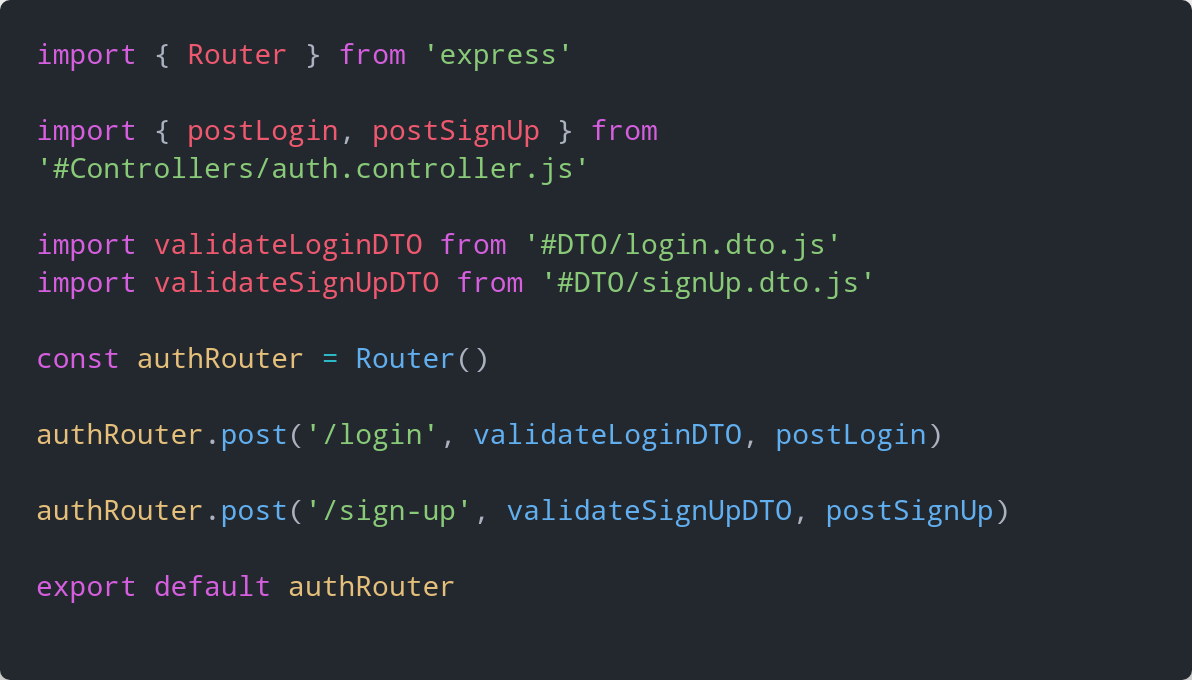
\includegraphics[width=1\textwidth]{img/auth-router}
  \caption{Router de autenticación}
  \label{fig:auth-router}
\end{figure}

\subsubsection{Controladores}
Los controladores son los encargados de realizar las funciones que se ejecutan al
realizar una petición a la API. En el caso de esta aplicación, se han creado
controladores para la autenticación, los usuarios, las obras de arte y los administradores,
cada uno con sus funciones correspondientes. Estas funciones son en realidad middlewares
que se encargan de realizar las acciones necesarias para cada petición.

Un middleware es una función que, como se explica en la documentación de \textit{Express}
\cite{express-middleware}, recibe por parámetros tres objetos:

\begin{itemize}
  \item \texttt{req}: objeto de petición (\textit{request}) que contiene la información
  de la petición HTTP.
  \item \texttt{res}: objeto de respuesta (\textit{response}) que contiene la información
  de la respuesta HTTP que se va a enviar.
  \item \texttt{next}: función que, al ejecutarse, ejecuta el siguiente middleware que se
  haya definido para esa ruta, ya que para una ruta se pueden ejecutar varios middlewares.
\end{itemize}

La nomenclatura utilizada para definir los distintos middlewares de los controladores es
la siguiente: \texttt{<tipoRequest><NombreFuncion>}. Donde \texttt{<tipoRequest>} es el
tipo de petición HTTP que se recibe (\texttt{GET}, \texttt{POST}, \texttt{PUT} o
\texttt{DELETE}) y \texttt{<NombreFuncion>} es el nombre de la función. Por ejemplo,
la función que se encarga de realizar el inicio de sesión de un usuario se llama
\texttt{postLogin} ya que es una petición \texttt{POST}. Todo esto se puede ver en la
imágen \ref{fig:auth-controller} donde se muestra el código del controlador de
autenticación.

\begin{figure}[H]
  \centering
  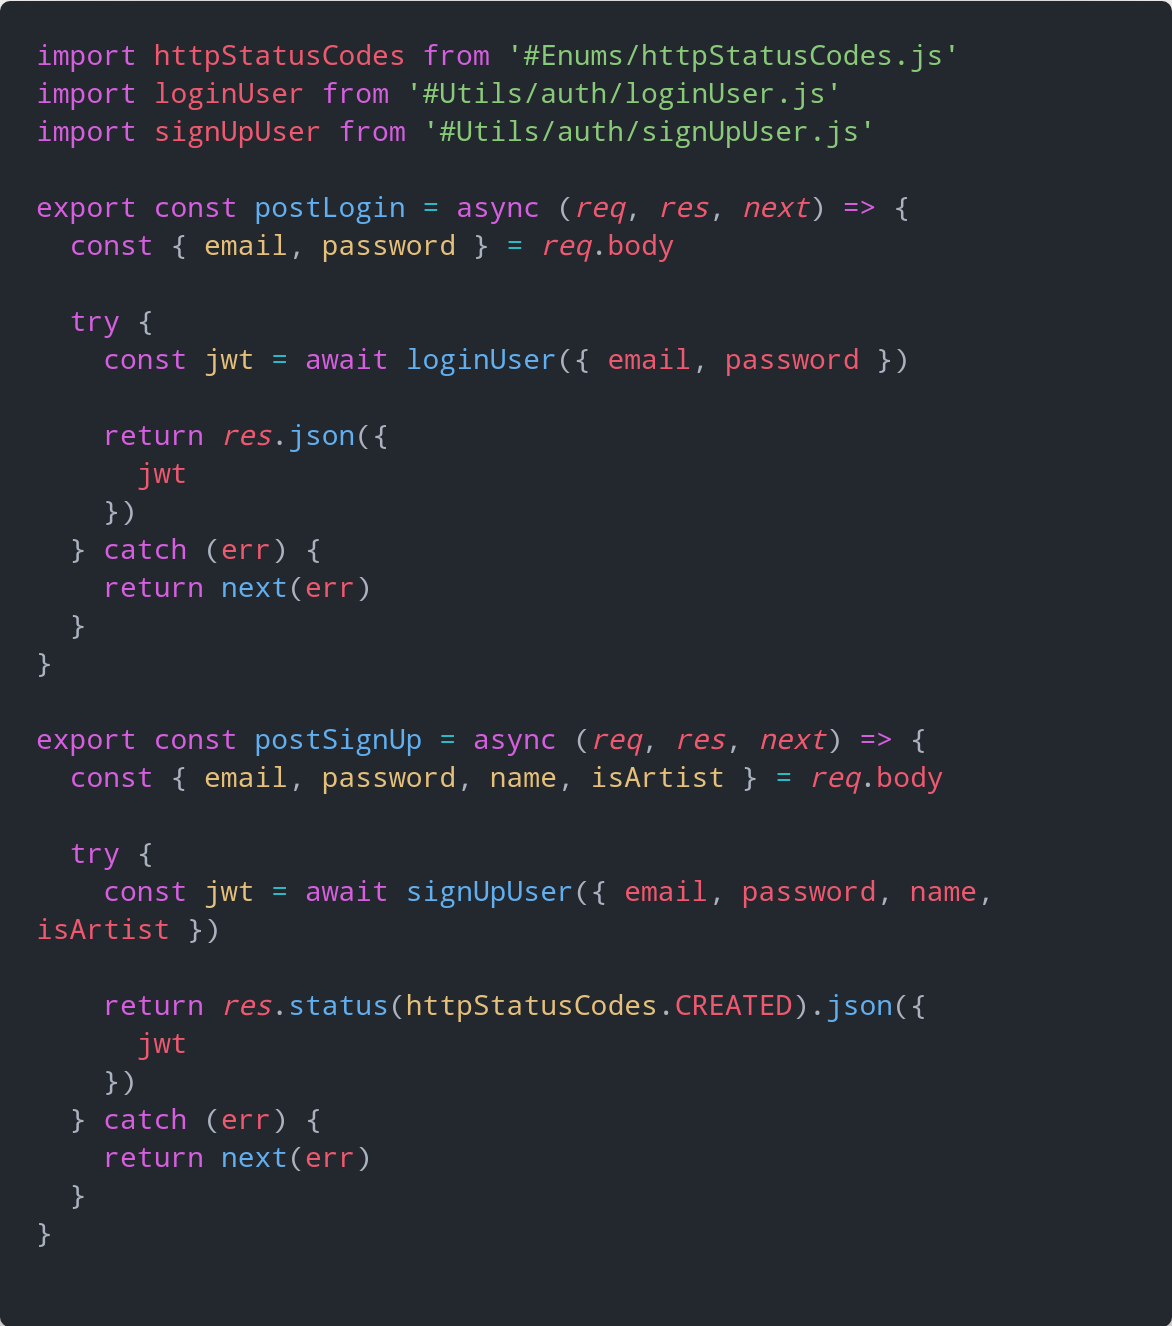
\includegraphics[width=1\textwidth]{img/auth-controller}
  \caption{Controlador de autenticación}
  \label{fig:auth-controller}
\end{figure}

En estas funciones podemos ver cómo en primer lugar se obtienen los datos del body de
la petición y no hace falta comprobar si existen o son correctos ya que de eso se ha
encargado el middleware de DTO (Data Transfer Object), que habíamos mencionado al hablar
de las rutas, y cuya ejecución es anterior al de la función del controlador.

A continuación, se ejecuta el código que corresponda y se devuelve una respuesta haciendo
uso del objeto \texttt{res} e indicando el código de estado de la respuesta HTTP y el JSON
que se va a devolver.

El código de la función se ejecuta dentro de un bloque \texttt{try/catch} para capturar
los posibles errores que se puedan producir y, con la función \texttt{next()}, se envían
dichos errores a los middlewares que se encargan de manejar los errores (son los dos últimos
middlewares que se pueden ver en la imágen de la app de \textit{Express}
\ref{fig:express-app}). Estos middlewares se encargan de devolver los errores en formato
JSON y con el código de error correspondiente, manteniendo siempre la misma estructura de
respuesta. Este manejo de errores es el que se propone en la documentación de \textit{Express}
\cite{express-error-handling}.

\subsubsection{DTOs} \label{sssec:DTOs}
Un DTO (Data Transfer Object) es un objeto que se utiliza para transferir datos entre
diferentes capas de una aplicación. Tal y como se explica en este artículo \cite{dto-validation},
los DTOs son una buena práctica para validar los datos que llegan en el body de una petición
HTTP.

Para el desarrollo de esta aplicación se ha utilizado la librería \textit{Ajv} \cite{ajv}
que permite definir un esquema de validación de los datos que llegan en el body de una
petición HTTP, pudiendo definir los tipos de datos que se esperan, si son obligatorios o
no y algunas validaciones adicionales como el tamaño de un string, si es un email válido,
si cumple una regex o si el valor del dato está en un enumerado, entre otras.

En la imágen \ref{fig:password-dto} se puede ver la definición de la propiedad
\texttt{password} del DTO de inicio de sesión y registro de usuarios. En ella se puede
ver que se espera un string, que es obligatorio y que tiene que tener una longitud mínima
de 6 caracteres, una longitud máxima de 50 caracteres y que tiene que cumplir una regex
que comprueba que la contraseña tenga al menos una letra minúsucula, una letra mayúscula y
un número. También se puede ver que se han definido mensajes de error personalizados para
cada una de las validaciones.

\begin{figure}[h]
  \centering
  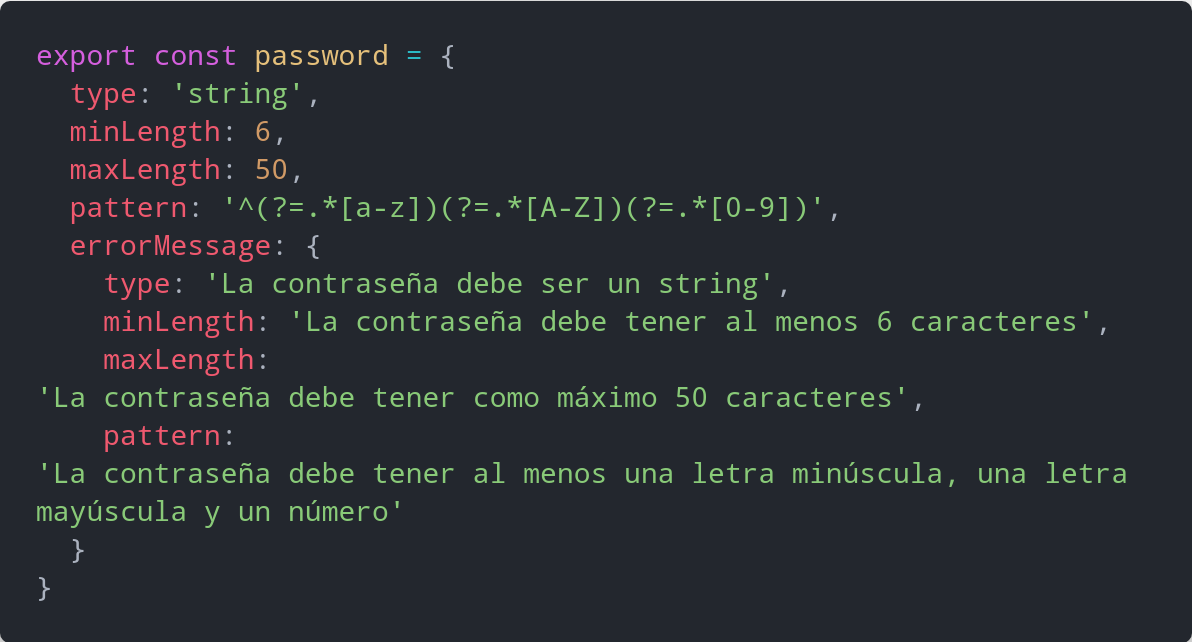
\includegraphics[width=1\textwidth]{img/password-dto}
  \caption{Definición de la propiedad \texttt{password} del DTO de inicio de sesión y registro}
  \label{fig:password-dto}
\end{figure}

Los esquemas de validación DTO se generan con una función auxiliar que se ha creado con este
propósito y se compila con la función \texttt{ajv.compile()} de la librería \textit{Ajv}
\cite{ajv-methods}. Con este esquema se crea un middleware que se ejecuta antes de las
funciones de los controladores y que se encarga de validar los datos que llegan en el body
de la request. Si los datos no son válidos, se devuelve un error con los mensajes de error
definidos en el esquema de validación correspondiente. Un ejemplo de esto se puede ver en
la imágen \ref{fig:auth-router} donde podemos ver los middlewares \texttt{validateLoginDTO}
y \texttt{validateSignUpDTO} que se ejecutan antes de las funciones \texttt{postLogin} y
\texttt{postSignUp} respectivamente.

\newpage

\subsubsection{Autenticación} \label{sssec:auth}
Para la autenticación de los usuarios en la aplicación se ha utilizado \textit{JWT}
\cite{jwt} que es un estándar basado en objetos \textit{JSON} para poder transmitir
información de forma segura y firmada digitalmente a través de un token. Se barajó la
opción de utilizar una autenticación basada en sesiones, pero se descartó porque
la autenticación mediante token es más segura y sencilla de implementar, como se
explica en este artículo \cite{token-vs-session}.

Para el manejo de los tokens se ha utilizado el módulo \textit{jose} \cite{jose} que
permite generar y verificar tokens \textit{JWT} \cite{jwt} mediante una serie de funciones.

Dado que junto con el token se puede enviar información encriptada para que el cliente
pueda acceder a ella, se ha decidido enviar el \textbf{id del usuario} y su \textbf{rol}.
Esto permite que desde el frontend se pueda saber de manera sencilla si el usuario está
autenticado y qué acciones puede realizar en la aplicación.

Para la firma del token se ha utilizado un \textit{secret} que se ha definido en una
variable de entorno en el \texttt{.env}. Este \textit{secret} se utiliza para verificar
que el token es válido y que no ha sido modificado. Todo este proceso se explica en la
documentación \cite{jose-sign}, donde se enseña también a encriptar con diferentes
algoritmos. En este caso se ha utilizado el algoritmo \texttt{HS256}. Además se ha
definido un tiempo de expiración del token de \textbf{8 horas}, tiempo tras el cual
el token dejará de ser válido y el usuario tendrá que volver a iniciar sesión.

Desde el frontend, cada vez que se realiza una petición a la API (que deba estar
autenticada), se envía el token en la cabecera de la petición siguiendo el estándar
\textit{Bearer} \cite{bearer}. Este token se verificará en el backend y, si es válido,
se ejecutará la función correspondiente de la petición, en caso contrario, se devolverá
un error de autenticación.

Para la autenticación de los usuarios se ha creado un middleware que se ejecuta antes
de las funciones de los controladores y que se encarga de verificar que el token que
llega en la cabecera de la petición es válido, utilizando la función \texttt{jwtVerify()}
\cite{jose-verify} de \textit{jose}.

Este middleware se puede ver en la imágen \ref{fig:auth-middleware}. En caso de que el
token sea válido, se obtiene el id del usuario y se añade al objeto \texttt{req}, después
se ejecuta la función \texttt{next()} para que se ejecute la función del controlador
correspondiente a la petición, donde se podrá acceder al id del usuario que se acaba de
almacenar en \texttt{req}. Si el token no se válido se envía el error de autenticación
con la función \texttt{next()} para que se ejecuten los middlewares de manejo de errores
explicados anteriormente.

\begin{figure}[H]
  \centering
  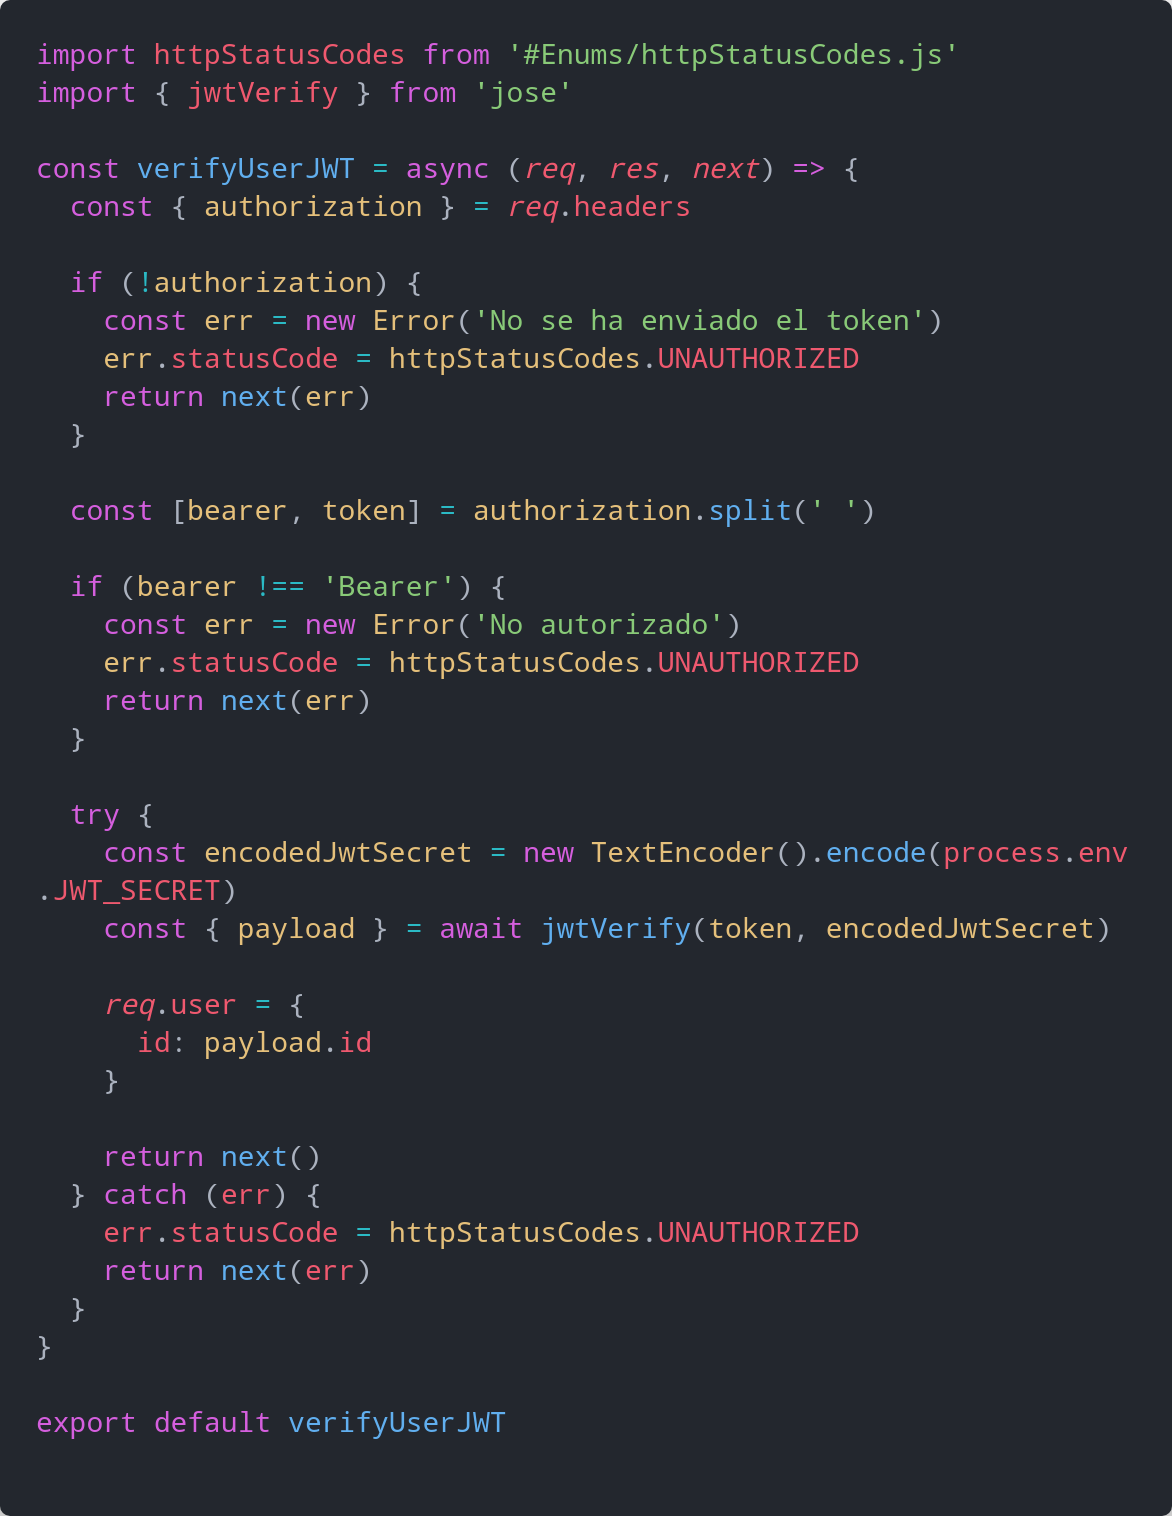
\includegraphics[width=0.8\textwidth]{img/auth-middleware}
  \caption{Middleware de autenticación}
  \label{fig:auth-middleware}
\end{figure}

\subsection{Frontend}

El frontend de la aplicación se ha desarrollado utilizando \textit{React} \cite{react}
y algunos componentes de \textit{Material-UI} \cite{material-ui}.

La aplicación de \textit{React} \cite{react} consta de un archivo \texttt{index.html}
que es el punto de entrada de la aplicación y donde se encuentra el elemento
\texttt{<div id=``root''></div>} en el cual se va a renderizar la aplicación. A nivel de
\textit{JavaScript} se tiene un archivo \texttt{main.jsx} que es el archivo desde el que
se inicia la aplicación y donde, a través del react-dom, se obtiene el elemento
\texttt{<div id=``root''></div>} mencionado anteriormente y en él se renderiza el componente
\texttt{App} que es el componente principal de la aplicación.

\subsubsection{Vite}

Para hacer el frontend de la aplicación se ha creado un proyecto nuevo usando
\textit{Vite} \cite{vite} que es una herramienta que facilita el desarrollo del frontend
de aplicaciones web. Consta de un servidor de desarrollo para poder ir viendo los cambios
que se van realizando en la aplicación en tiempo real y de un \textit{bundler} que se
encarga de compilar el código con todas sus dependencias.

Se ha utilizado \textit{Vite} \cite{vite} en lugar de \textit{Create React App}
\cite{create-react-app}, que era la herramienta que se utilizaba anteriormente por defecto
para crear proyectos de \textit{React} \cite{react}, porque es más rápido y por su
manejo de las dependencias. Además, en la documentación oficial de \textit{React}
\cite{start-react-project} ahora recomienda utilizar \textit{Vite} \cite{vite} para crear
nuevos proyectos si no vamos a utilizar un framework completo.

En las imágenes \ref{fig:vite-bundle} y \ref{fig:vite-esm} \cite{why-vite} se puede ver la
diferencia entre lo que se hace tradicionalmente con \textit{bundlers} para el desarrollo y
lo que hace \textit{Vite} \cite{vite}, que es utilizar el sistema de módulos de JavaScript
(\textit{ESM}) \cite{esm} para importar los módulos dinámicamente en el navegador. Esto
agiliza mucho el proceso de desarrollo evitando tener que compilar el código cada vez que
se realiza un cambio.

\begin{figure}[H]
  \centering
  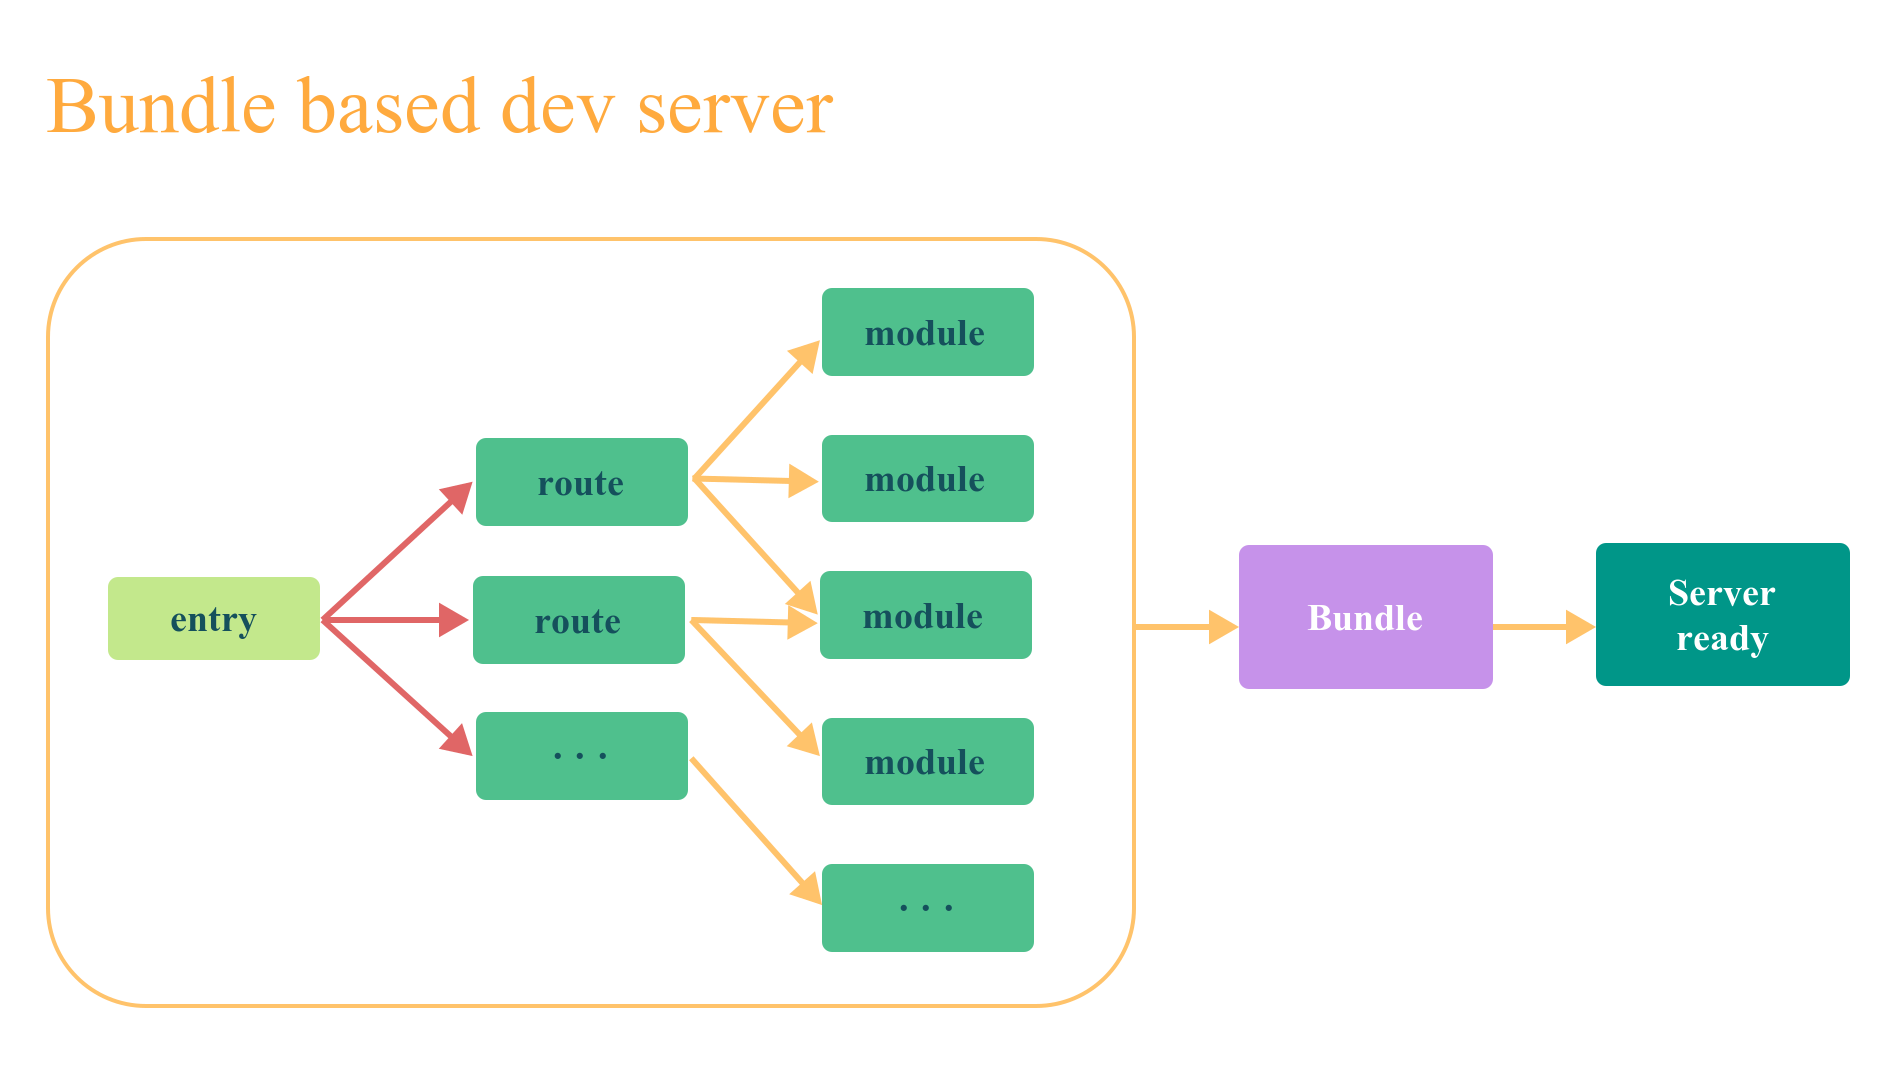
\includegraphics[width=1\textwidth]{img/bundle-based}
  \caption{Proceso de desarrollo con \textit{bundlers} \cite{why-vite}}
  \label{fig:vite-bundle}
\end{figure}

\begin{figure}[H]
  \centering
  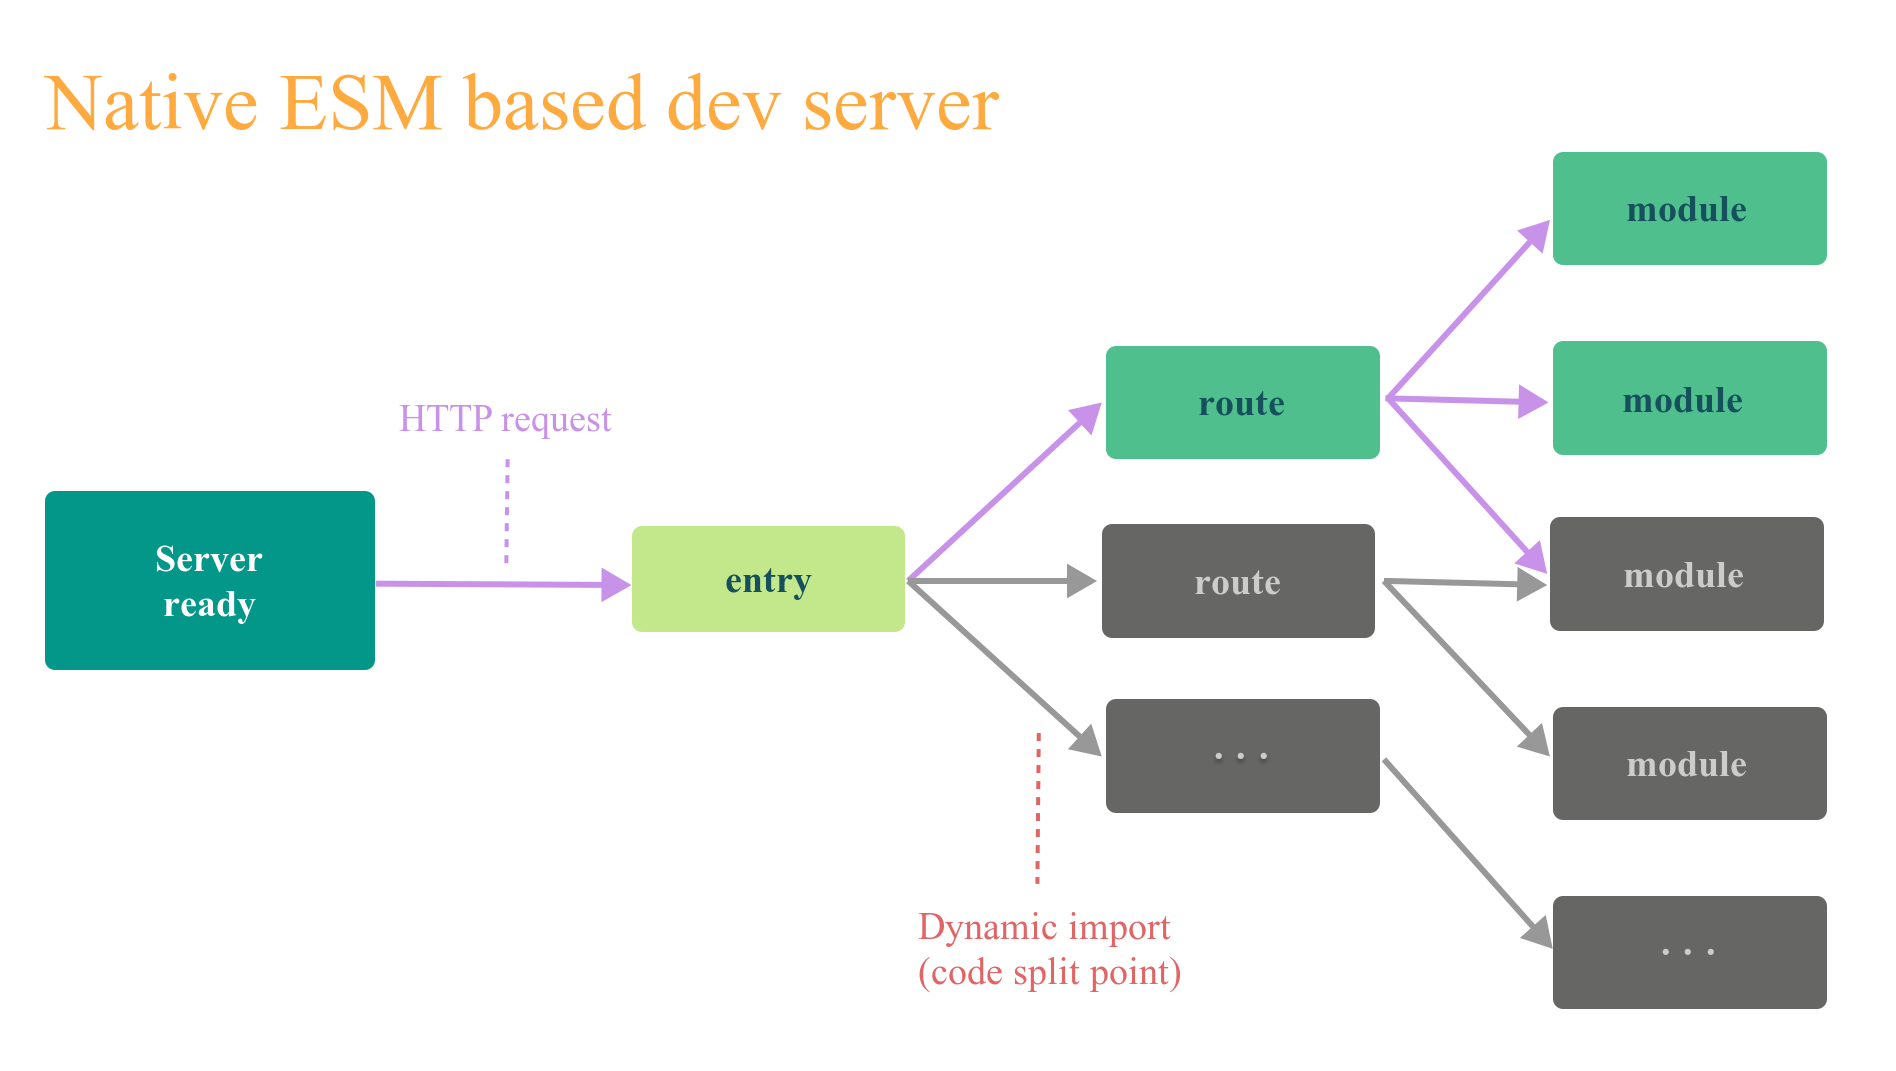
\includegraphics[width=1\textwidth]{img/esm-based}
  \caption{Proceso de desarrollo con \textit{ESM} \cite{why-vite}}
  \label{fig:vite-esm}
\end{figure}

Se ha utilizado también \textit{SWC} \cite{swc} que es un compilador de JavaScript y
TypeScript que es más rápido que \textit{Babel} \cite{babel} y que se integra con
\textit{Vite} \cite{vite} con un plugin que han desarrollado \cite{vite-swc}, afirmando
que es hasta 20 veces más rápido que \textit{Babel} \cite{babel}.

\subsubsection{Rutas}
Para gestionar las rutas de la aplicación se ha utilizado \textit{React Router}
\cite{react-router} que es la librería más utilizada para este propósito.

Se ha usado el componente \texttt{BrowserRouter} y se ha seguido la documentación
\cite{browser-router} para definir las rutas de la aplicación. En la imágen
\ref{fig:app} se puede ver el componente \texttt{App} que es el componente principal
de la aplicación y donde se definen las rutas de la misma.

Como se puede observar, se define el \texttt{AuthProvider} (que se explicará más adelante)
y dentro de él se define el componente \texttt{Routes} que es el que se encarga de
definir las rutas de la aplicación.

La primera ruta tiene \texttt{path='/'}, que es la ruta raíz por lo que todas las rutas
renderizarán el componente que se le pasa como valor a la prop \texttt{element}, el
componente \texttt{Layout}. Este componente es el que tiene la estructura principal de la
aplicación, que tiene que estar presente en todas las páginas. Consta de un \texttt{header}
con la barra de navegación y un \texttt{main} donde se renderiza el componente
\texttt{Outlet} \cite{outlet} que se encarga de renderizar el \texttt{element}
correspondiente a la ruta hija que se esté visitando.

La última ruta, con \texttt{path='*'}, es la ruta por defecto que se renderiza cuando
no se encuentra ninguna otra ruta que conicida con la ruta que se está visitando en la
aplicación.

\newpage

\begin{figure}[H]
  \centering
  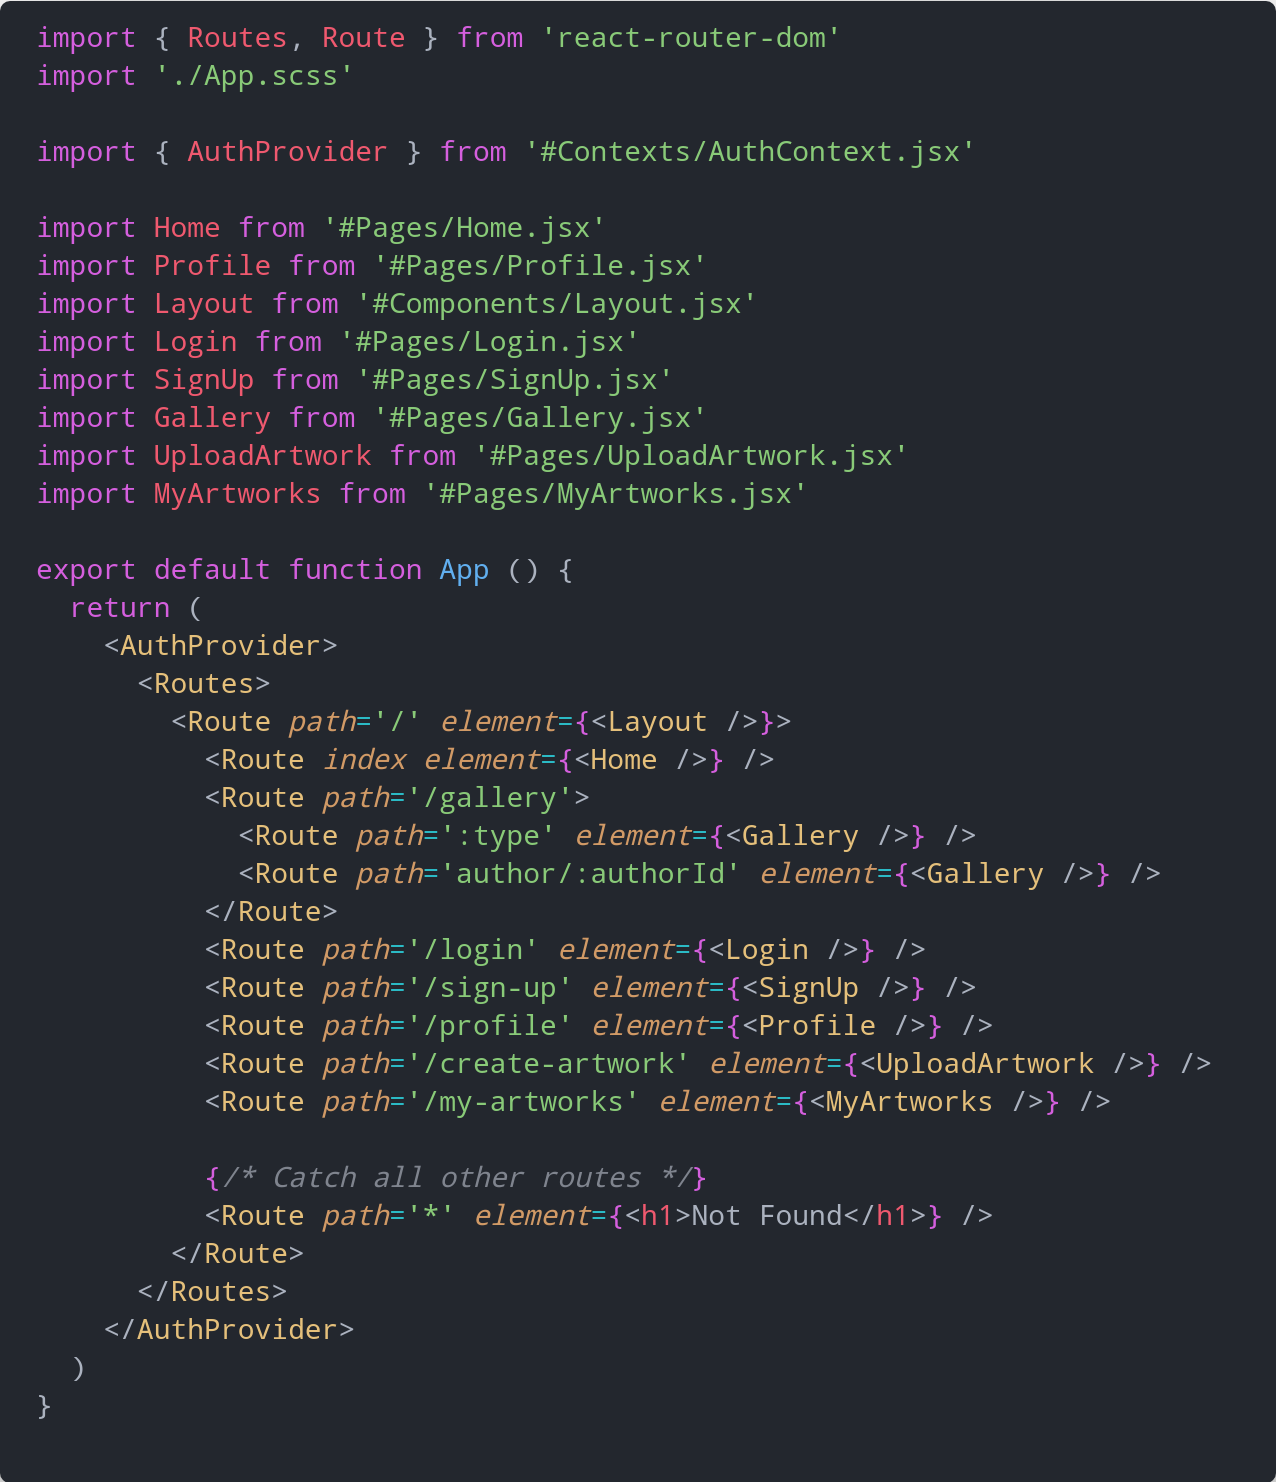
\includegraphics[width=1\textwidth]{img/app}
  \caption{Componente \texttt{App}}
  \label{fig:app}
\end{figure}

\newpage

\subsubsection{Contexto de autenticación} \label{sssec:AuthContext}
Para gestionar la autenticación de los usuarios en el frontend se ha utilizado el
\textit{hook} \texttt{useContext} \cite{use-context} de \textit{React} \cite{react},
que permite suscribirse a un contexto previamente definido y acceder a él desde cualquier
componente hijo de dicho contexto.

Para esto se ha definido el contexto \texttt{AuthContext} con la función
\texttt{createContext} \cite{create-context} de \textit{React} \cite{react} y se ha creado
un componente \texttt{AuthProvider} que es el que se encarga de gestionar el estado de la
autenticación de los usuarios. Este es el que se puede ver en la imágen \ref{fig:app}
englobando al resto de componentes de la aplicación. Esto permite que este contexto esté
disponible en toda la aplicación.

En el componente \texttt{AuthProvider} se definen los estados \texttt{user} y
\texttt{token} que son los que se van a utilizar para guardar la información de
autenticación del usuario, en caso de ser nulos, significa que el usuario no está
autenticado. También se definen las funciones \texttt{setAuth} y \texttt{deleteAuth} que
se encargan de guardar y eliminar la información de autenticación del usuario en el
\textit{localStorage} \cite{local-storage} del navegador.

\subsubsection{Componentes}
Los \textbf{componentes} son la base que utiliza \textit{React} \cite{react} para
construir las interfaces de usuario \cite{react-component}. Los componentes son como
funciones que engloban el marcado \textit{HTML}, los estilos \textit{CSS} y la lógica
\textit{JavaScript} de una parte concreta de la interfaz de usuario. Los componentes
devuelven un código \textit{JSX} \cite{jsx} muy similar al \textit{HTML} y es el que
se renderiza en el navegador. Los componentes pueden tener propiedades que se pasan
como parámetros desde el componente padre.

En la aplicación se han creado algunos \textbf{componentes} en la carpeta \texttt{pages}
que son los que se renderizan al visitar una ruta de la aplicación. Estos componentes
suelen ser componentes padres que engloban a otros componentes más pequeños que se
encargan de renderizar partes más concretas de la página. Estos componentes más pequeños
se han creado en la carpeta \texttt{components} y también pueden tener componentes hijos
que se renderizan dentro de ellos.

Para manejar la lógica de los componentes se han utilizado los \textbf{estados} de
\textit{React} \cite{react-state} que son como variables de los componentes que se
mantienen entre renderizados y que, al ser modificados, hacen que el componente se
vuelva a renderizar, permitiendo así que se actualice la interfaz de usuario.

\subsubsection{Estilos}
Para los estilos de la aplicación se han escrito en \textit{SCSS} \cite{scss} y se han
utilizado algunos componentes de \textit{Material-UI} \cite{material-ui} como, por ejemplo,
el componente \texttt{Rating} \cite{rating} para mostrar las valoraciones de las obras o
el componente \texttt{Modal} \cite{modal} que se utiliza para mostrar los detalles de una
obra de arte de la galería. Además, este último componente se ha anidado dentro de otro
\texttt{Modal} para mostrar todas las valoraciones y comentarios de una obra de arte.

\subsubsection{Hooks}
Los \textbf{hooks} son una característica de \textit{React} \cite{react-hooks} que
permite usar distintas funciones de \textit{React} \cite{react} en los componentes.
Por ejemplo el \textit{hook} \texttt{useState} \cite{use-state} para manejar los
\textit{estados} de los que se ha hablado anteriormente o el \textit{hook}
\texttt{useContext} \cite{use-context} para poder acceder a un contexto como se ha
explicado en la sección anterior, sobre el contexto de autenticación \ref{sssec:AuthContext}.

Además, \textit{React} \cite{react} permite crear \textbf{hooks personalizados} que
llaman \textbf{custom hooks} \cite{custom-hooks}. Estos permiten encapsular una lógica
que se vaya a utilizar en varios componentes. En la aplicación se han creado algunos
\textbf{custom hooks} como el hook \texttt{useAuth} que se encarga de obtener la
información de autenticación del usuario del contexto de autenticación o el hook
\texttt{useErrors} que se encarga de gestionar los errores que se pueden producir en los
componentes. Este último se muestra en la imágen \ref{fig:use-errors} donde se puede ver
que se define un estado \texttt{errors} para almacenar los errores y dos funciones:
\texttt{saveErrors} que se encarga de guardar los errores en el estado y \texttt{clearErrors},
encargada de limpiar los errores del estado.

\begin{figure}[H]
  \centering
  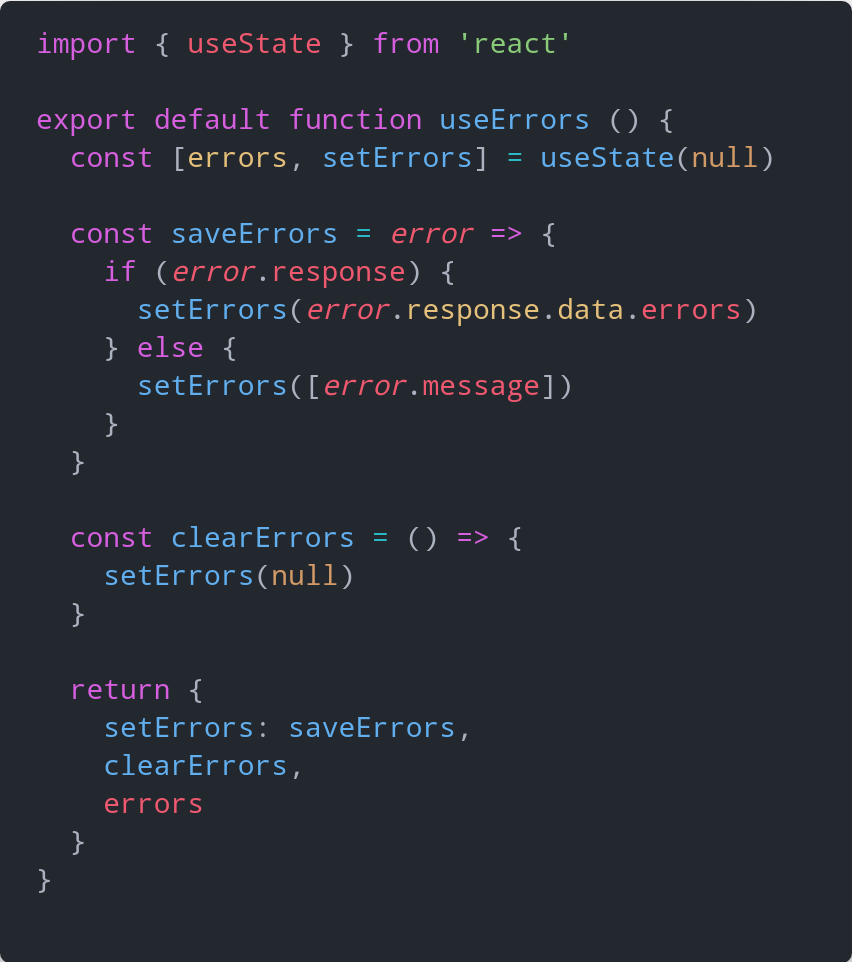
\includegraphics[width=0.6\textwidth]{img/use-errors}
  \caption{Hook \texttt{useErrors}}
  \label{fig:use-errors}
\end{figure}

\subsubsection{Servicios}
Para realizar las peticiones \texttt{HTTP} a la API se han creado unos servicios que
se encargan de esta labor. Se han creado tres servicios, uno para las peticiones relacionadas
con la autenticación, otro para las peticiones relacionadas con los usuarios y otro para
las relacionadas con las obras de arte.

Las peticiones se realizan mediante la librería \textit{Axios} \cite{axios} que permite
realizar peticiones \texttt{HTTP} de manera sencilla. La configuración de \textit{Axios}
\cite{axios} es muy sencilla, simplemente se crea una instancia indicando la \texttt{baseURL}
de la API. Esto se ha realizado en un archivo de configuración \texttt{axios.js} que devuelve
la instancia del cliente de \textit{Axios} \cite{axios} evitando así tener que crear una
instancia en cada servicio.

La instancia de \textit{Axios} \cite{axios} cuenta con los métodos \texttt{get},
\texttt{post}, \texttt{put} y \texttt{delete} que son los que se utilizan para realizar
las peticiones \texttt{HTTP} a la API. A estos métodos hay que pasarles como primer
parámetro la ruta de la petición, como segundo parámetro los datos que se quieran enviar
en el body de la petición (en caso de que sea necesario) y el último parámetro es un objeto
con la configuración de la petición como, por ejemplo, los \textit{headers}.

En la imágen \ref{fig:create-artwork-service} se puede ver la función \texttt{createArtwork}
del servicio de obras de arte que se encarga de realizar una petición \texttt{POST} a la API
para crear una obra de arte. En ella se puede ver que la función recibe como parámetro un
objeto con los datos de la obra de arte y el token de autenticación del usuario. Se utiliza
el método \texttt{post} de la instancia de \texttt{axiosClient} pasándole como primer
parámetro la ruta de la petición, como segundo los datos con los que se quiere crear la obra
de arte y como tercer parámetro los \textit{headers} de la petición, que en este caso son
el \textit{header} de \texttt{Authorization} con el token en el formato \texttt{Bearer}, tal
y como se explicó en la sección \ref{sssec:auth}; y el \textit{header} de
\texttt{'Content-Type': 'multipart/form-data'} que es el que se recomienda cuando se envían
datos con archivos, como es el caso de las obras de arte \cite{multipart-form-data}. Por
último, se devuelve la respuesta de la petición.

\begin{figure}[H]
  \centering
  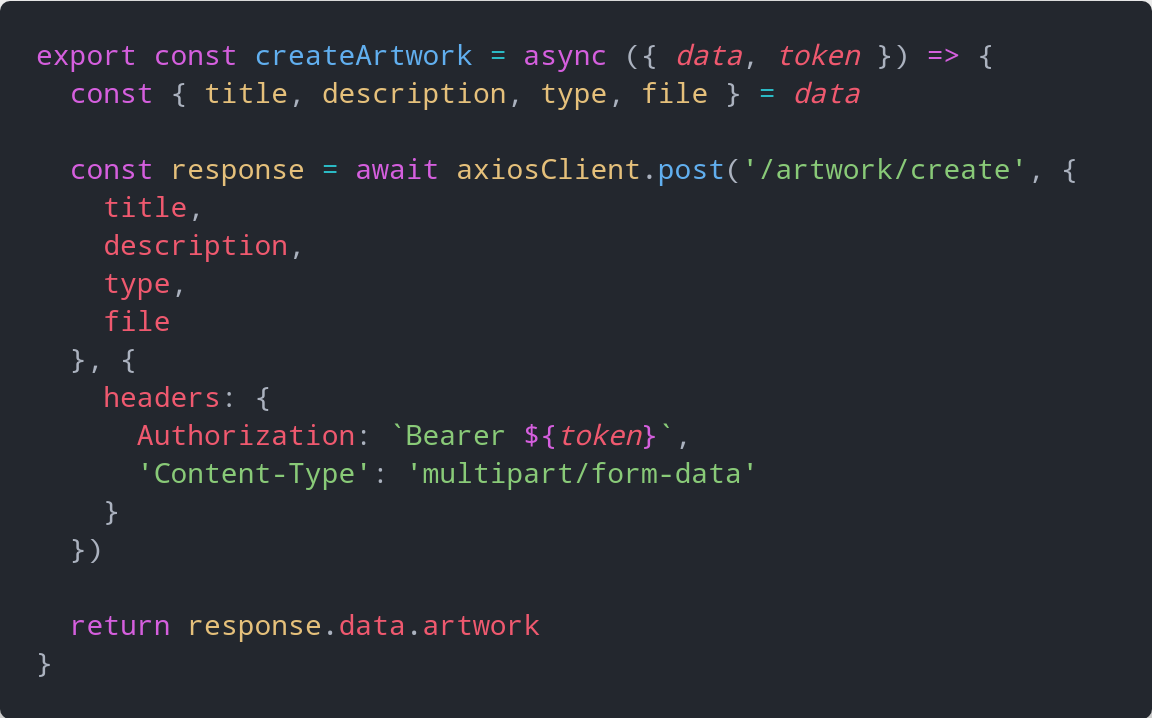
\includegraphics[width=1\textwidth]{img/create-artwork-service}
  \caption{Función \texttt{createArtwork}}
  \label{fig:create-artwork-service}
\end{figure}

\subsection{Despliegue}
Para el despliegue y conexión de todas las partes de la aplicación se ha utilizado
\textit{Docker} \cite{docker} que es una plataforma que permite crear, desplegar y ejecutar
aplicaciones dentro de contenedores. Estos contenedores son un \textbf{entorno de
virtualización} ligero y aislado que permite ejecutar aplicaciones independientemente del
sistema operativo en el que se ejecute. A diferencia de una máquina virtual, los contenedores
no necesitan un sistema operativo virtualizado para funcionar, sino que utilizan los recursos
del sistema operativo del host y solamente virtualizan los componentes necesarios para
ejecutar la aplicación y sus dependencias. Estos contenedores son \textbf{independientes del
sistema operativo} y entre ellos, por lo que podemos evitar así problemas de dependencias o
conflictos entre aplicaciones aunque se ejecuten en el mismo host.

Para el despliegue de la aplicación se ha utilizado \textit{Docker Compose}
\cite{docker-compose} que permite definir y ejecutar multiples contenedores de \textit{Docker}
\cite{docker}. En el caso de esta aplicación, se han definido cuatro contenedores: uno para
la base de datos, otro para \textit{PhpMyAdmin} \cite{phpmyadmin}, otro para el backend y
otro para el frontend.

Tanto el backend como el frontend se han definido con un \textit{Dockerfile} \cite{dockerfile}
que es un archivo que contiene instrucciones para crear una \textit{imagen} de \textit{Docker}
para crear el contenedor. En ambos, se ha utilizado como base la \textit{imagen} oficial
de \textit{Node.js} \cite{nodejs-docker} en su versión \texttt{18-alpine} que está basada en
\textit{Alpine Linux} \cite{alpine-linux} (una distribución muy ligera de Linux). Además,
en estos \textit{Dockerfiles} se copian los archivos necesarios del host de la aplicación al
contenedor y se instalan las dependencias de la aplicación con el comando \texttt{npm install}
de \textit{npm} \cite{npm}.

La base de datos se ha definido directamente en el \textit{docker-compose.yml} usando la
\textit{imagen} oficial de \textit{MySQL} \cite{mysql-docker} en su versión \texttt{8.0}
y definiendo las variables de entorno necesarias para la configuración de la misma.

Para el gestor de base de datos se ha utilizado la \textit{imagen} oficial de
\textit{PhpMyAdmin} \cite{phpmyadmin-docker} en su última versión y también se han definido
las variables de entorno necesarias para su conexión con la base de datos.